\begin{figure}
    \centering
    \begin{subfigure}[b]{0.45\textwidth}
        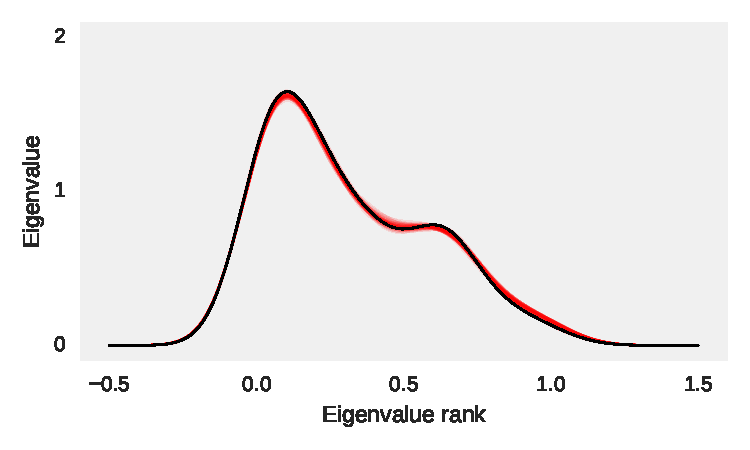
\includegraphics[width=\textwidth]{FishPoo/figures/gopher_louse_spectral_density_permutations}
        \small
        \caption{Permuted spectral densities}
    \end{subfigure}
    \begin{subfigure}[b]{0.45\textwidth}
        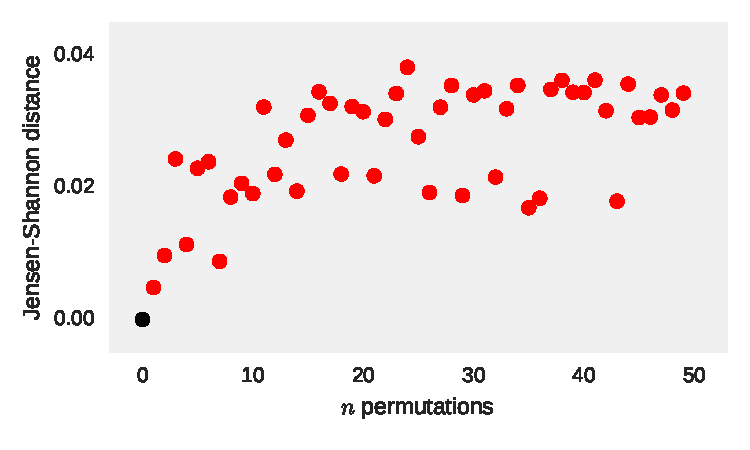
\includegraphics[width=\textwidth]{FishPoo/figures/gopher_louse_spectral_density_permutation_distances}
        \small
        \caption{Shannon-Jensen distances}
    \end{subfigure}
    \caption{Spectral density distributions of successively permuted interactions among pocket gophers and their chewing lice parasites from Hafner {\em et al.} \cite{hafner1994disparate} \textbf{(a)} and the Shannon-Jensen distances between each with respect to the spectral density distribution of the un-permuted interaction \textbf{(b)}.}
    \label{fig:FP_permuted_distances}
\end{figure}